\documentclass[12pt]{article}
\usepackage[utf8]{inputenc}
\usepackage{verbatim}
\usepackage{caption}
\usepackage{float}
\usepackage{geometry}
\usepackage{graphicx}
\usepackage{gensymb}
\author{John Scott and Oliver Thomas,\\Bristol QECDT}
\title{Optical Jigsaw Instructions}
\begin{document}
\maketitle

\section{Description}

The Optical Jigsaw is an outreach demo used to demonstrate guiding light using differences in refractive indices and repeaters.

\section{Introduction/Narrative}

Transmitting information using light forms the basis of nearly all modern communications, including the internet. This demo is a small scale (toy) copy of the things you need to talk to someone so far away that it would take you 10 hours to travel there but you can have a conversation with them in real time! 

We are using light to send our message, light is a great carrier of information as it is the fastest thing in the universe. Most of the world uses fibre optic cables which are under water on the ocean floor. Fibre optic cables are made of glass which is close to the width of a human hair.

In our demo we are using a type of plastic (perspex) which has very similar properties but on a much larger scale. We use lightpipes to guide light around, similarly to how water flows through pipes. The proper name for them are waveguides, but lightpipes sounds more fun! The light is contained inside the optical fibre or lightpipe due to total internal reflection.

\begin{figure}[h]
\centering
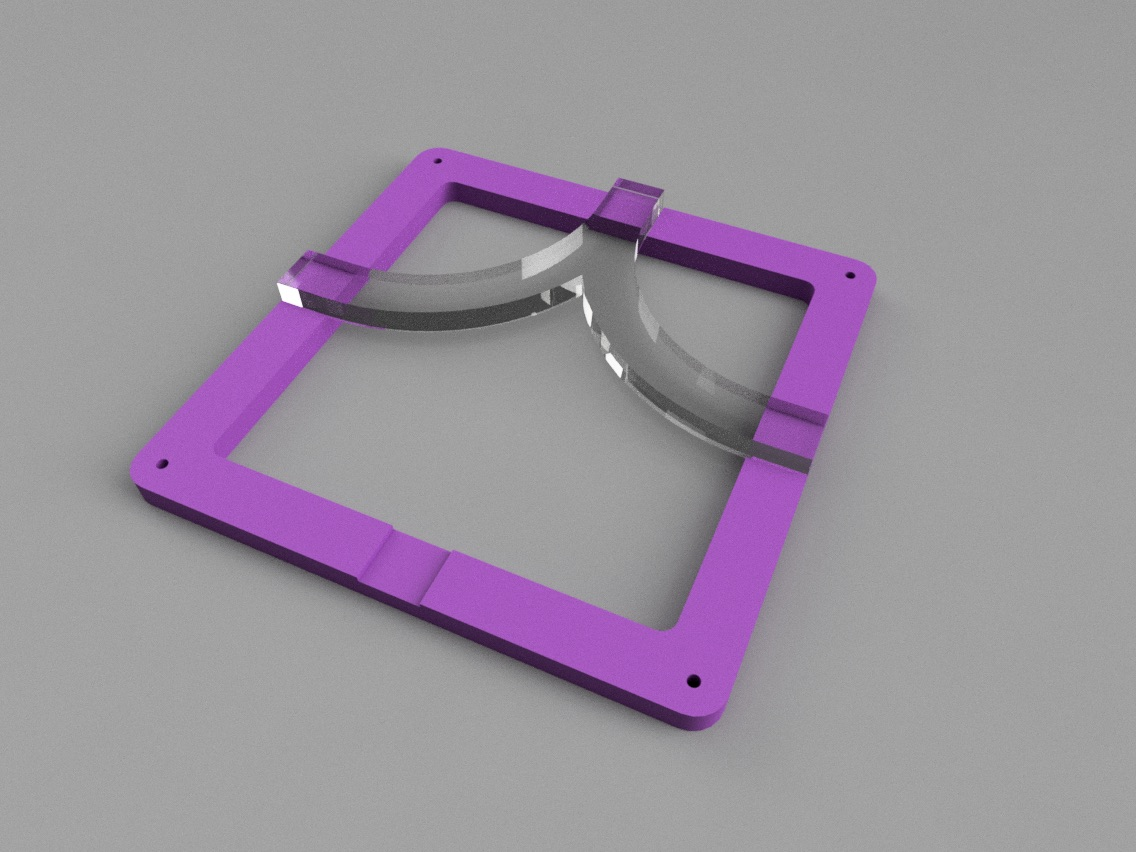
\includegraphics[width=0.45\textwidth]{figures/jigsaw_y-junction.jpg}
\caption{Splitter}
\end{figure}

You can do some pretty nice things using lightpipes. There are straight and curved sections, and we can also split the light into two paths. In fact the lightpipes here are bigger versions of some of the components that make up a quantum computer. A quantum computer is a new type of computer which will be able to solve problems no other computer can.

The problem with guiding light is that the light leaks out of the lightpipes. You can see this as the lightpipes get dimmer after each block. We use a repeater to make the light brighter.  

The object of the demo is to get light from one end to the other using the lightpipe blocks.

\section{User instructions}

\begin{itemize}
    \item The rechargeable torches (micro-usb) work best as sources. There are a few torch holder
        frames. Use fishing wire or string to hold the torches.
    \item Each board uses two PP3 (9 volt) batteries. Each repeater lasts between 6-10 hours using a single non rechargeable battery (rechargeable batteries don't last as long. It's a good idea to have quite a few batteries on hand). There is an on-off switch on each board. Keeping the boards off when not in use saves the batteries
    \item Due to an issue with back-reflection causing the repeaters to trigger
      themselves we have taken out the LDRs (light dependent resistors) on one side of each of
        the repeaters, meaning they are now only one-directional.
    \item Each LED on the repeaters has a POT (potentiometer) associated to it. Tuning
        the POT tunes the sensitivity to incoming light. There are arrows next to each
        POT which point to the LED it tunes.
    \item The demo works best in dark or constant light-level rooms, otherwise frequent
        tuning is needed to ensure the LEDs trigger properly.
    \item We found that each repeater worked for around 3 blocks. The corner pieces and
      crossers are very lossy.
    \item Handle the repeater boards by the frame not the electrical circuit board (the green PCB) because they're fragile.
\end{itemize}


\section{Troubleshooting}

\textbf{If a repeater isn't working,}
\begin{enumerate}
\item Check the switch is on.
\item Check it is facing in the correct direction. The light should be shining on the LDR side (turn it round if it isn't).
\item Reduce the number of lightpipes between the repeater and the source.
\item Try tuning the POT all the way through its range of both directions until the LED turns on. The POT clicks at the end of its travel.
\item Check the batteries are charged up.
\end{enumerate}
%
\textbf{If a torch isn't working,}
\begin{enumerate}
    \item Check the torch is on. The button is on the bottom of the torch
    \item Try plugging in the torch as the battery is probably flat. You can charge it from a laptop via USB.
\end{enumerate}


\section{Risks}
\begin{itemize}
\item The device is 9V battery powered so there are no electrical safety issues
\item The LEDs are quite bright but not dangerous. It is uncomfortable to look directly into the LEDs
\item The plastic pieces may have sharp corners (but we didn't find any).
\item The repeater pieces are quite delicate and might be damaged if dropped. Broken pieces might have sharp corners.
\end{itemize}

\begin{comment}
Box outline with waveguides inside, 
\begin{verbatim}
---------------
|             |
|_____________|
|_____________| 
|             |
|             |
---------------

---------------
|     |  |    |
|     |  |    |
|     |  |    | 

|     |  |    |
|     |  |    |
---------------

\end{verbatim}

We want to be able to tile the squares together to create a maze. We are also including curved sections (not shown here).

\end{comment}



\newpage
\section{Improvements to be made}

General areas for improvement
\begin{itemize}
	\item Fix back reflection triggering a permanent loop using a microcontroller.
	\item Redesign the repeaters to work in all four directions on the square enabling 90\degree turns 
	\item Reconfigurable directions
	\item Button to autotune background light level
	\item PWM magic
	\item Mains power supply 
	\item Colour filters
	\item Change voltage regulator/supply
	\item Wireless support
	\item Pots for current control giving adjustable brightness/power consumption	
\end{itemize}
Some possible suppliers and costs:
\begin{itemize}
	\item allpcb 10 100x100mm pcbs 2mm thickness \$75.
	\item Perspex for 1000x1000mmx2mm £40
        \item Possible chip: PIC18F1230
\end{itemize}

In order to produce a DXF autocad schematic we will use FREECAD which is avaliable on the ubuntu repository.

We want to have around 15mm thickness in the perspex waveguides and they should fit on 150x150mm$^2$ blocks


\end{document}